\section{Convergence of the Method}
\label{sec:convergence}

The above halo-based metrics will have a certain level of dependence on the
choice of halo finder used. In an attempt to ensure independence of the results
from such factors, the above analysis was repeated both with the 3D
friends-of-friends (FoF) halo finder included in the {\tt yt} package \citep{Turk2011}.
We also repeated the analysis with the \velociraptor{} 6D FoF finder.
The latter will disentangle active mergers, but as active mergers make up a small
fraction of the galaxy population, the above results are qualitatively
unaffected and are only change quantitatively to the 5\% level.
The use of a FoF finder, rather than the spherical overdensity finder found
in AHF, did not qualitatively change the results.

In the below, we discuss ways to extend the lagrangian region definition to include
more particles, whilst still retaining the ability to have non-uniform shapes. We
find that, in general, including more particles in the definition of the lagrangian
region (than are present in the halo) leads to a fractionally higher level
of inter-lagrangian transfer and more self-contribution to the final halo mass
at the expense of transfer from outside any lagrangian region. This is expected, as
now many more particles are classified as being present in the lagrangian region.


\subsection{Filling in Holes}


One valid criticism of our methodology for producing lagrangian regions is that
they are relatively spotty; simply using the dark matter particles from a given
halo naturally leads to a very diffuse lagrangian region. To remedy this, it is
possible to smooth out the lagrangian regions, by extending the procedure
that was used to extend the regions from the dark matter to the gas.
This works as follows:
\begin{enumerate}
	\item For every dark matter particle that does not end up in a halo 
	      in the initial conditions, find the nearest $n$ neighbours.
	\item Find among the neighbours the maximal lagrangian region ID,
	      corresponding to the lowest mass $z=0$ halo.
	\item Assign the particle the same lagrangian region ID.
\end{enumerate}
The choice to assign the particles to the lowest mass halo, rather than the
higher mass halo, was made to ensure that spurious transfer into the lower mass
halo was avoided wherever possible. This means that the expectation is that
with this metric the level of inter-lagrangian transfer will increase with
respect to the fiducial lagrangian region identification method. The results
with the particles given to the halos of a higher mass show negligible
deviation from the fiducial result.

\begin{figure}
	\centering
	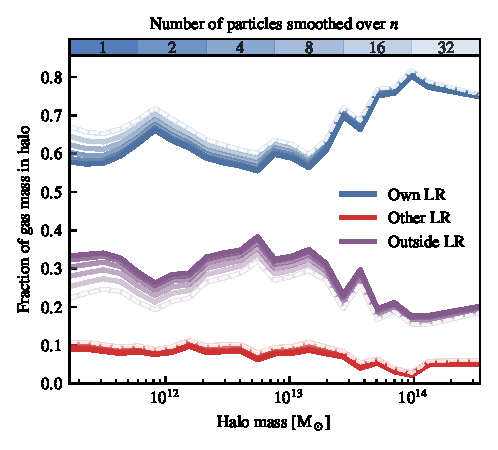
\includegraphics{figures/convergence_smoothing.pdf}
	\vspace{-0.7cm}
	\caption{The gas transfer mass function reproduced from Fig.
     \ref{fig:maintransferresult}. Each line, coded by transparency, shows the
     fraction of baryonic mass in a halo from each component when the lagrangian
     regions have been smoothed by 1 (i.e. the fiducial result), 2, 4, 8, 16, or
     32 particles (from darkest to lightest respectively). The white dashed line
     shows the result for the 32-smoothing case where the particles are given to
     the highest, rather than lowest, mass halos; no difference is seen here
     suggesting that there is little overlap between the lagrangian regions on
     these scales. See the text for the details of how this smoothing is
     constructed.}
	\label{fig:smoothconv}
\end{figure}

The results are shown in Figure \ref{fig:smoothconv}. Note how smoothing the
lagrangian regions does have the expected effect of inducing more internal
transfer, and does increase the proportion of baryons that are classified as
retained as the lagrangian regions are filled out. Despite this, the overall
trends with respect to halo mass remain.

\subsection{The sizes of halos}

The `size' of a halo is always a choice that is imposed, with larger or
smaller halo radii (as long as these are consistent between halos) also being
completely valid characterisations of the halo mass and size. In Figure
\ref{fig:bigtransferpic} we saw that there was a large amount of gaseous matter
inside halos from outside any lagrangian region. It may be reasonable to assume
that this gas corresponds to dark matter that is simply sitting just outside of
the halo edge, perhaps within the so-called `splashback radius'. The estimates
for this radius range between 0.8 and 1.5$R_{\rm vir}$ \citep{More2015}, and hence
below we consider the situation where we extend the region around the halo that
contributes to the lagrangian region. This is done in the following way:
\begin{enumerate}
	\item For every halo, find its current virial radius $R_{vir}$. This contains
	      all particles at redshift $z=0$ that we consider to be within the halo.
	\item Increase this to $R_{\rm LR}$, and find all dark matter particles within
		  this region. These dark matter particles are now defined to lie within
		  the lagrangian region of that halo.
	\item ID match these particles and extend to the gas in the usual way.
\end{enumerate}
We chose this specific process, increasing the radius of our lagrangian region
rather than the whole halo, to prevent us from simply re-defining our halo size
and including more gas as well (as in this case, the transfer across the halo
boundary would simply be moved to a larger radius). The effects of this process
on the gas component of the BTMF (where it is most significant) are shown
in Figure \ref{fig:radius_dependence}.

\begin{figure}
    \centering
    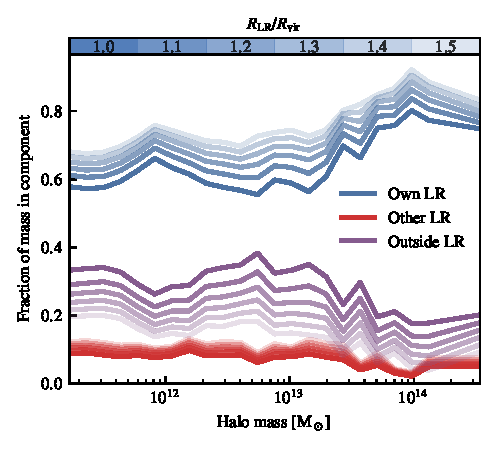
\includegraphics{figures/radius_convergence.pdf}
    \vspace{-0.7cm}
    \caption{Convergence with increasing virial radius for the lagrangian region.
    Lighter colours correspond
    to large radii, going in steps of $0.1R_{\rm vir}$ from 1.0 to 1.5.}
    \label{fig:radius_dependence}
\end{figure}

Here we see that there is a significant change in the fraction of mass in the
halo at redshift $z=0$ from outside any lagrangian region, especially when going to
$R_{\rm LR} = 1.5 R_{\rm vir}$. This large change is expected, though, as we now
have included a volume that is three times larger than the initial halo in the
lagrangian region classification; taking this extreme value for all halos
really is a `worst-case' scenario. The inter-lagrangian transfer remains at a similar level
despite the increase in radius. Note that there will be no extra mass included in the
halos here, with particles simply changing their lagrangian allegiances.